% 
% POSTMORTEM ANALYSIS DOCUMENT 
% ================================
% 
% Time-stamp: <2010-03-26 04:52:04 raskolnikov>
% (c) 2009 The JAGSAT development team.
% 

\documentclass[12pt,a4paper]{article}

\usepackage{raskolnikov}

\title{\large JAGSAT project\\\huge Bussiness Plan}
\author{
  Juan Pedro Bolívar Puente\\ 
  Aksel Junkkila\\
  Guillem Medina\\ 
  Sarah Lindstrom\\ 
  Alberto Villegas Erce\\ 
  Thomas Forss
}
\location{Project Course \\ \textit{Åbo Akademy}}
% \date{}

\begin{document}
\maketitle

\begin{center}
\textbf {Revision history}

\begin{tabular}{ l | l | l | l }
Date			&Version	&Description		&Author\\\hline\hline
09.03.2010	&1.0		&Creation 		&Sarah Lindstrom\\
22.03.2010	&1.1		&LaTeX Format	&Alberto Villegas
\end{tabular}
\label{tab:rev}
\end{center}

\vfill
Copyright 2009 AUTHORS.
Permission is granted to copy, distribute and/or modify this document under the terms of the GNU Free Documentation License, Version 1.1 or any later version published by the Free Software Foundation;  with no Invariant Sections, with no Front-Cover Texts, and with no Back-Cover Texts. A copy of the license is included in the ``D9: Licenses''  document entitled `GNU Free Documentation License''.

\pagebreak
\tableofcontents
\pagebreak

\section{Executive summary}
Our business idea is about developing electronic board games for different touch screen devices. The games will be multiplayer games which can be played on touch screen devices. The device can be placed on for example a kitchen table and the game can be played like a traditional board game. Our main idea is to develop mostly traditional, but also new games that can be experienced in a new way, on a new device.

The feeling of playing together with your friends and family, which is the core of board games, will still be there, only now you will be able to use the latest technology. We want to deliver a game play update so that the old games can be enjoyed in a more modern way but also give new games the technology they deserve. With electronic board games there is only storage space needed for the device you play the games on. The days when you needed to stash ten different game boxes in your closet are behind you! With electronic board games you only need one device.

The market segment we are focusing on at the moment is young adults with or without children. Although, since there are so many different games to be played there are possibilities for both adults and children to enjoy game playing on the touch screen devices. More about this in the market section.

There are many other competitors out there developing games for touch screen devices, but not that many are now focusing on traditional board games. We believe that we therefore have a competitive advantage in this market.  Our team is also very innovative and are experienced in both developing and playing computer and board games; something we believe is very important when developing games. Our team consists of six masters degree students. Five of us focus mainly on development, while one of us is business oriented.

\section {The JAGSAT Project}
\subsection{Team members}
The team consists of six students at Åbo Akademi University. Three of us are here through an exchange program that Åbo Akademi University has with some universities in Spain. The rest of us are students at Åbo Akademi University. Five of us are studying in the field of Computer Science, while one of us is in the field of Information Systems.

\begin{tabular}{ | l | l | }\hline
Sarah Lindstr\"om			&Business consultant\\
Thomas Forss				&Project manager/Programmer\\
Aksel Junkkila				&Game designer\\
Alberto Villegas			&Documentation manager/Programmer\\
Guill\'em Medina			&Programmer\\
Juan Pedro Bol\'ivar Puente	&Main programmer\\\hline
\end{tabular}

We are all participating in a project course at Åbo Akademi University. This project is active from September 2009 until March 2010. We are all interested in the game industry and when TribeFlame introduced the opportunity to develop an electronic board game, we formed this group.

\subsection{Our goal with the JAGSAT project}
We want to develop old as well as modern games, focusing on the social aspect of the gaming experience. Consoles are a very popular component in homes today and people are always looking for new ways of interacting with each other. Social games like SingStar, Buzz, Rockband and different movement based games for Nintendo Wii are constantly entering the market. We believe that electronic board games can be complete this picture.

\section{Competitive edge}
\subsection{The business idea}
Our business idea is about developing electronic board games for different touch screen devices. Traditional board games today are made from an old concept with boards, paper money and/or different cards to play with. We believe there could be a great market for developing electronic board games and update the board game environment. Consumer friendly touch screen devices are really booming in 2010 and we want to offer yet another reason to buy one!

\subsection{What's new?}
Games have been played on touch screen devices for quite many years now, but to be able to play traditional board games on the devices is something new. Social games are all around us these days for example Sing Star, Rockband and different kinds of quiz games. There are even board games versions for consoles, like Monopoly for the xbox 360. Though many social games exist today, they can only be played on consoles or PC. With electronic board games, we are really focusing on the social part of social gaming and introducing a new way of playing traditional board games with a new device.

\subsection{Purpose of product}
First and foremost, the games will in general satisfy a social need for the players. With the electronic board games they can interact with each other and play face-to-face. In today's world, face-to-face interaction is not that common any more, which we believe will make the customers choose this gaming experience in stead of buying a console game for socializing purposes. We don't want board gamers to have to give up cool and modern technology just because they want to play traditional board games.

Since we are developing all kinds of games this means that it is not a single product with one purpose. Except for the socializing part, each game will satisfy different needs for different customers. For example, if the game is chess the need of the player may be to have a quiet evening with his/her spouse over a glass of vine whilst playing chess. If the game is monopoly, many players can be involved and fight the whole night over who will win the game. Despite the different needs each game will satisfy, the social experience is the main need we want to satisfy by our electronic board games.

Because of this we also believe that our electronic board games will be played by a wide range of people. Both young and old are interested in board games and we believe that many of these will welcome a new way of playing. The older board gamers will appreciate that the social aspect is still very much present. The younger customers will be attracted by the new technology as well as being able to play new versions of the traditional board games.

\subsection{How unique is the business idea?}
There are many companies out there developing games for touch screen devices, the majority of them concentrating on mobile applications. The market for touch screen devices is soon about to explode and so we have from the start taken future competitors into consideration.

When we started this project, we could not find anyone else making electronic board games for touch screen devices. Now, with the release of Apples new iPad tablet, there has been some talk about Apple introducing electronic board games (Recombu 2010). The iPad is a good device for electronic board games. Since we are developing games for any touch screen device we welcome these devices on the market and believe that electronic board games will give customers another reason to buy one.

The Human Media Lab (\url{http://www.humanmedialab.org}) has also come up with a new technology they call "electronic board games". This works with "e-paper tiles that are tracked by a computer vision and operated through a projector" (Vizworld 2010). Although this device supports electronic board games, we think it can be expensive and not at all practical to use at home.

Other competitors are developers of social games played on consoles. People may want to buy a console on which they also can play other kinds of games (First-person-shooter games for example), instead of a touch screen device. The risk is that they won't think a touch screen tablet can be as versatile as for example a Play Station 3.

Another competitor are the traditional board games. People may think a touch screen device is too expensive for the purpose of playing board games on it (of course, this depends on the device, many of the devices soon to enter the market have many different functions). Though, for social gaming, we believe the "electronic board game experience" will be very appreciated.

\subsection{Our sustainable edge}
If we succeed in being the pioneers in this field, we have the advantage of being "king of the hill". Customers will associate electronic board games with us and not with other competitors. We are also developing games suitable for different kinds of touch screen devices, which opens up for a big market with many opportunities since the market for tablets are on the rise.

\section{Market}
In this chapter we will discuss the market we are about to enter. We will evaluate the size of the market as well as the market development. In this chapter we will also present out ideal customer and the pricing of our product. At the end of this chapter we will give a description of how we are planning to enter the market and which distribution channels we are going to use.

\subsection{Estimate and size of overall market}
The video gaming market is one of the biggest markets worldwide, even bigger than music and movies. Pricewatercoopers (PwC) has estimated that the global video gaming market will reach \$68,3 billion in 2012, with an annual growth rate of 10,3\% . The revenues for video games has also constantly increased from \$21,88 billion in 2002 to \$41,90 billion in 2007 (see appendix under section Sales figures for further information). Other sources estimate the market to expand to \$68,40 billion by 2012, which is also totally in line with the estimate made by PwC (Ars Technica, 2010).

Since our first game will be featured on the TribeFlame online store, for download or purchase, we are not at this moment restricting our market to for example Finland. It all depends on the success of the TribeFlame device and their online store. If it's a success and the news spreads, we can easily consider the Nordic countries, or even Europe, our market. We can of course at a later point make our game available also in other online stores.

\subsection{Market development}
While the video gaming (or interactive entertainment) industry is constantly growing (as mentioned above), the market for touch screen devices and consumer friendly tablets is  exploding right now. Since you need to own a touch screen device to play our games, we find it appropriate to also consider the tablet market in our business plan.

Apples iPad sales alone are estimated at 3-4 million devices sold in 2010 and 8 million in 2011 (Apple Insider, 2010). Other tablets are also hitting the market this year, like the Microsoft's Tablet PC, Lenovos IdeaPad tablet, HP Slate and Sony Dash (About.com, 2010). Even though some of these are not quite big enough to play electronic board games on, it shows that the market for consumer oriented tablets is going to explode this year. The TribeFlame device is of course the touch screen device on which we will run our first game. More information on the tablets mentioned here can be found in the appendix.

\subsection{Our ideal customer}
The paying customer are someone who already has some kind of a touch screen device on which he or she can play electronic board games. This means that the customer also has to have a relatively well payed job so he or she can afford a touch screen device or a tablet.

As already stated above, we are focusing on young adults with or without children. Our typical customer is a male or female in their 30's wanting to play board games with their spouse/friends/children. According to the 2008 report of the Entertainment Software Association (ESA) 59\% of gamers play games together with another gamer present. 66\% of the parents also believe that playing video games together with their children is a great way to socialize with the them. This shows that people are very much interested in the social aspect of gaming and want to play games together.

ESA also stated in their 2008 report that the average game player age is 35, which fits our ideal customer profile very well. ESA also reported that the adult gamers have on average been playing video or computer games for 13 years. This means that though they have 13 years of experience of playing, a 35 year old still remember playing traditional board games. We believe that customers with this experience combination will be the most attractive segment.

We have focused on young adults because we believe they are they ones that will most likely be interested in both the new technology and the board gaming experience. As they grew up the personal computer became more and more popular in the everyday home and along with it came computer games. The young adults are no stranger to computers or technical development. Now we can combine the board game experience they remember from their childhood with new cutting edge technology.

\subsection{Pricing}
Our games will not be expensive. The first game we are developing at the moment is a strategic war game based on the existing game Risk. The goal is to also incorporate a tower defense game that emerges during the fighting scenes. We are developing this game for a start-up company in Turku, Finland called TribeFlame. TribeFlame are developing the hard ware component for electronic board games. The device will be a multitouch touch screen device that can be used mainly for playing board games. The device will also be able to connect to the Internet, which means you can access the TribeFlame store and download (or buy) games from there. Our first game will be free or cost a maximum of five euros, this is not yet decided. Later on we will reconsider the pricing of our games. One alternative could be to offer re-makes of old board games for 0-10 euros and charge a bit more, maybe up to 30 euros, for a new game. Our main goal with the pricing is to be able to offer electronic versions of games to a cheaper price than the original ones.

\subsection{Similar products out there}
As mentioned above, when we started this project we could not find any developers of electronic board games. With the introduction of Apples new iPad tablet this discussion has risen. In the next couple of months we believe many direct competitors will emerge as a result of the tablet market booming. Since we are only developing the software, we are not threatened by the "tablet market". We are planning on offering our electronic board games to a wide range of touch screen devices after we have completed our first game for TribeFlame. We are of course keeping our eyes open for other developers of electronic board games for tablet devices.

\subsection{Distribution channels}
Concerning the hardware, there are many suitable devices entering the market at this point by manufacturers like Microsoft, Apple, HP and Sony (see appendix for pictures). We do not have a specific hard ware device in mind when developing games, but we are willing to do modifications so that the games will suit different kinds of devices. The most likely scenario is that the games will be available at an online game store, from where they can be downloaded. As mentioned, the game we are developing for TribeFlame at the moment is going to be available on the TribeFlame online store.

\subsection{Market entering}
We are now developing our first electronic board game for a start up company in Turku, Finland called TribeFlame (please see more information about TribeFlame under the chapter 5 Business partners). Our game will either be available for download or purchase (max five euros) at the TribeFlame online store. Our goal is to develop a combination of two old board games: Risk and traditional tower defense. We are developing this game for TribeFlame to support their new touch screen board game device. We are keen to see how customers will react to our game and after that we will continue to develop electronic board games.

\subsection{Marketing through social media}
Social media is a today a powerful tool when it comes to marketing you product, company or brand. Most of the social media marketing channels are also free of charge. Facebook now has over 400 million active users worldwide (Facebook Statistics) and Twitter 75 million (The Inquirer 2010). At the moment we have a page on Facebook (\url{http://www.facebook.com}) and Twitter (\url{http://www.twitter.com}). They are linked together so that we can share our status updates more easily.

\begin{figure}[H]
  \centering
  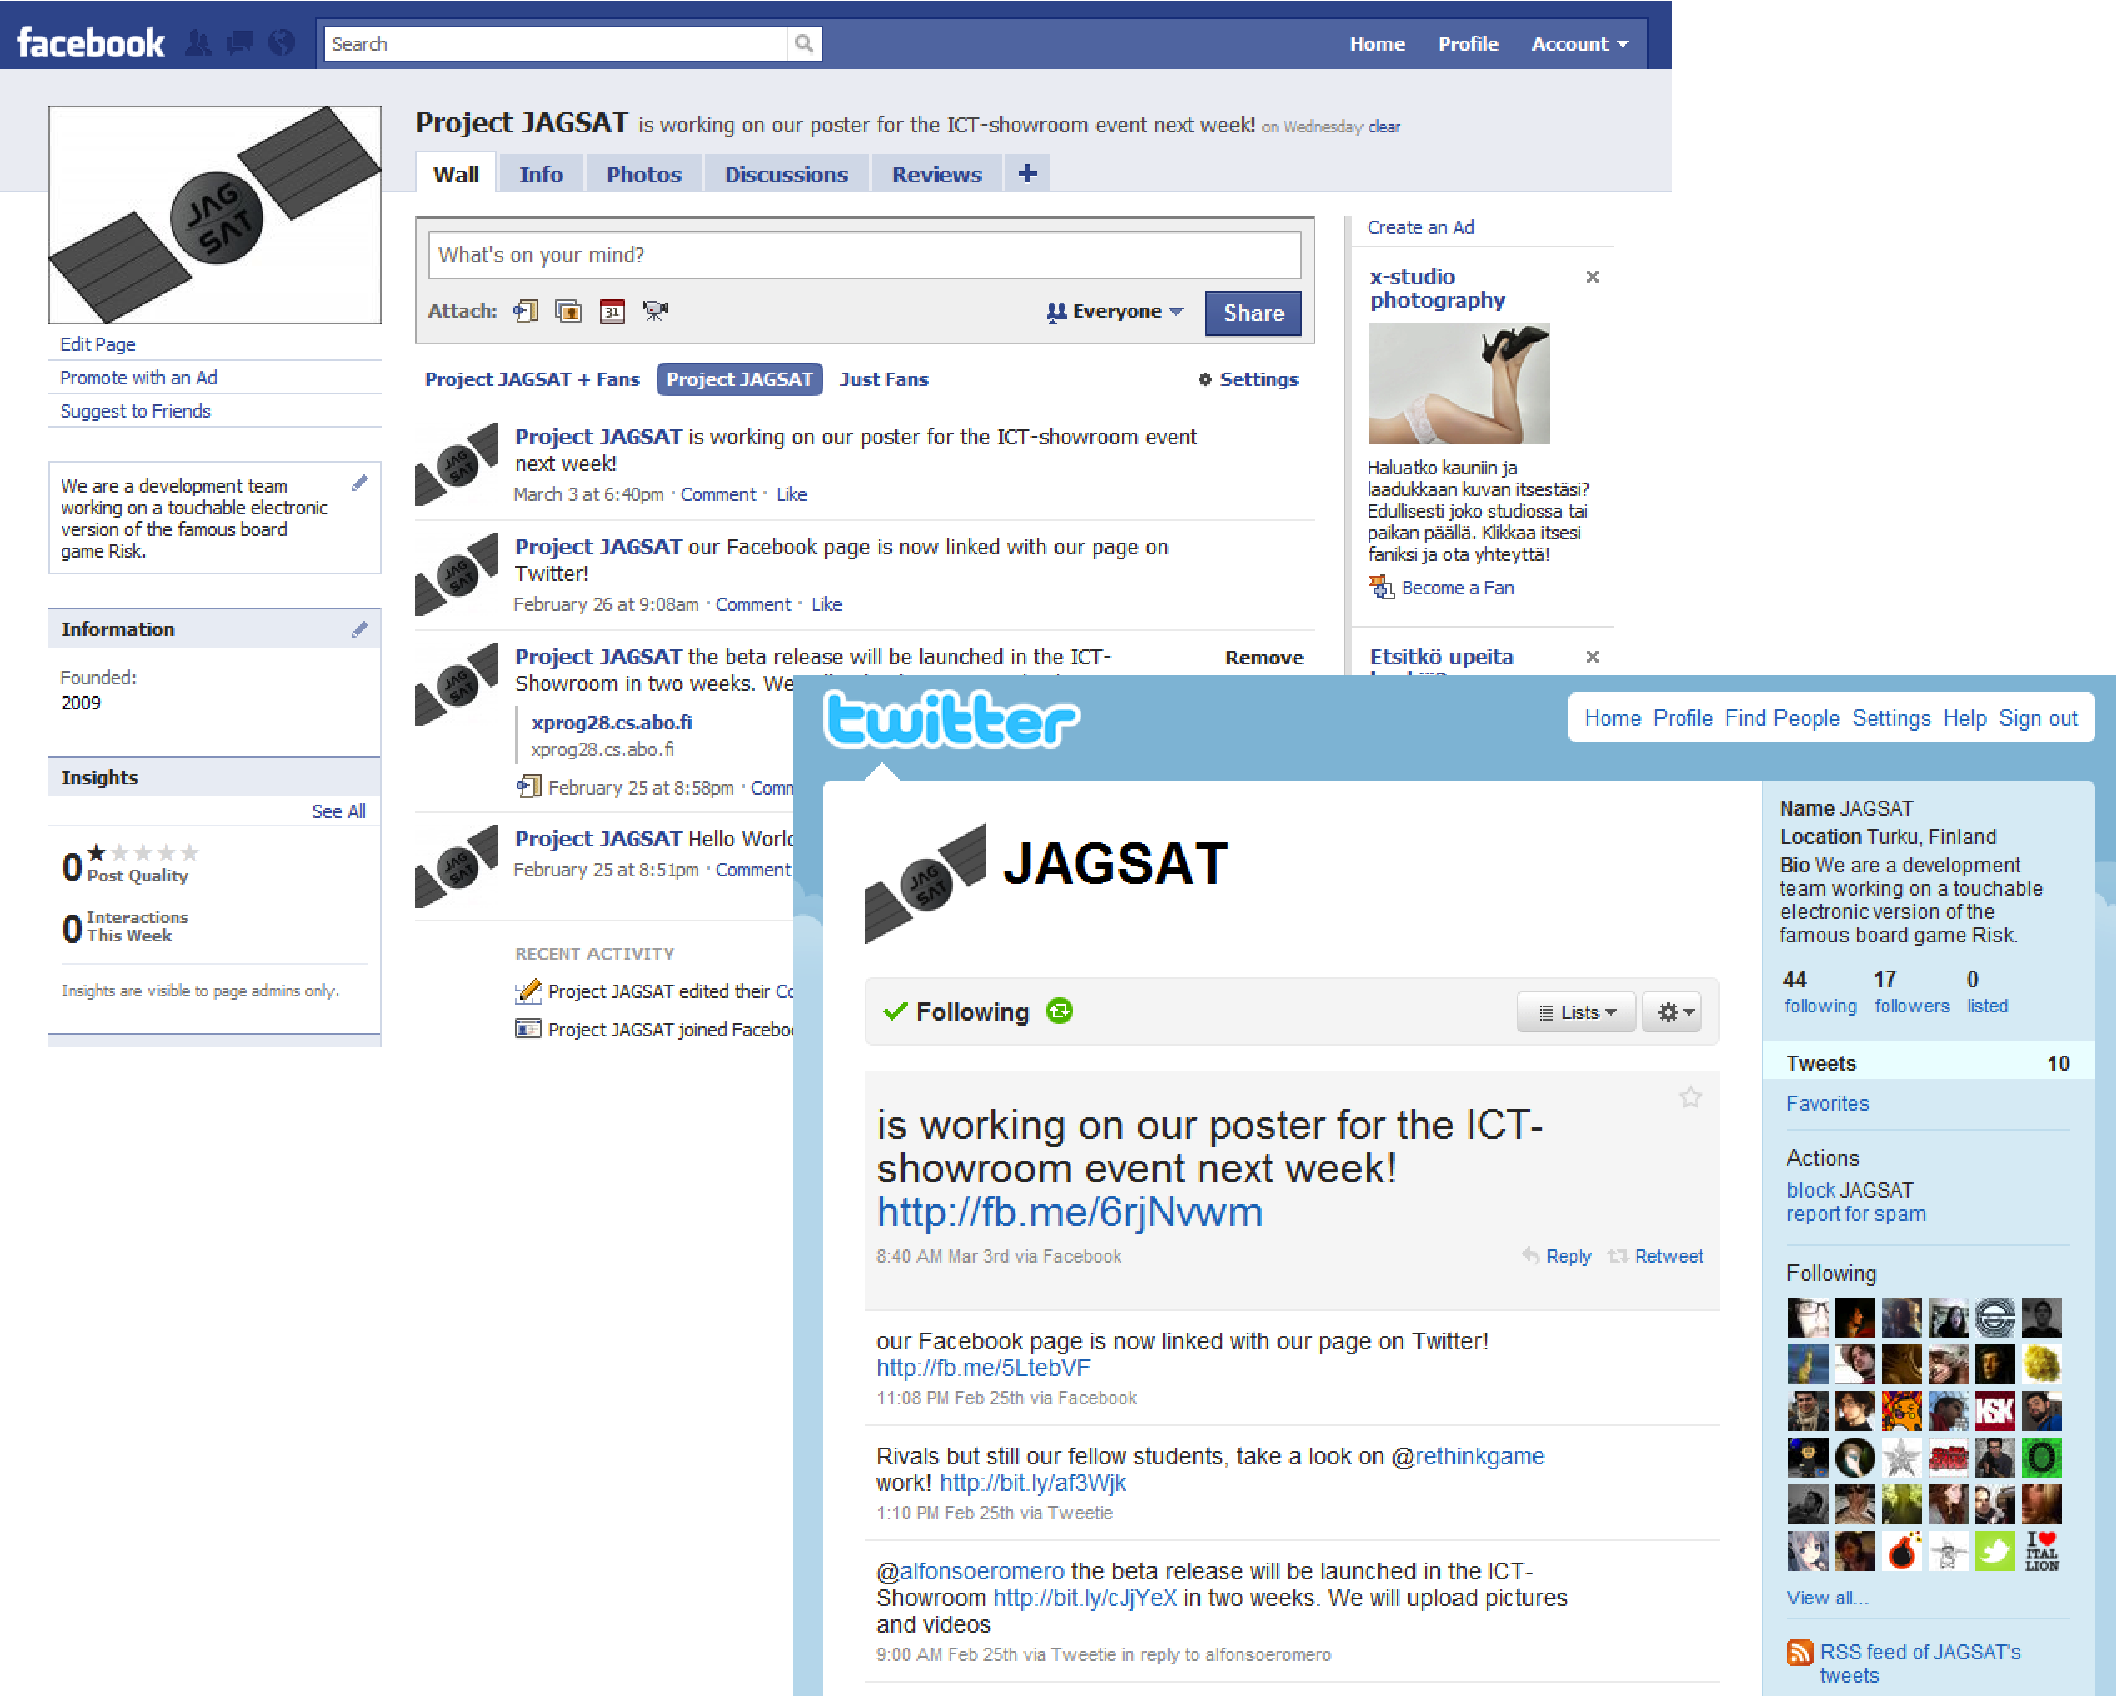
\includegraphics[width=12cm]{pic/bplan_01.pdf}
  \caption{Marketing through social media}
  \label{fig:mark}
\end{figure}

By using social media we are relying on "word of mouth" and since both communities are free of charge we believe that this is a good marketing channel for our first game and also for building a brand.

Later on we are planning on using social media to investigate what kind of games our users are interested in, what kind of features they would like to have etc. Using social media is a great tool for having a discussion with your customers and making sure you are developing something that they will actually buy.

\subsection{Business partners}
At the moment we are developing our first game for a new company called TribeFlame. TribeFlame are focusing on making a touch screen device ideal for electronic board games. Our first game will be designed for this device. In the future we will also design games suitable for other touch screen devices. TribeFlame will have an online store where you can buy games for their touch screen device. Our first game can be downloaded from there for free (or at a price of maximum five euros). As we develop more electronic board games we will focus on other online stores and other touch screen devices and tablets.

By working together with TribeFlame we are supporting their business as well as they are supporting us. TribeFlame need more games for the device they are developing and for us this is a chance to easily make our first game available for the public. Even if our game is free we are expecting it to get publicity and be recognized as one of the first developers of electronic board games.

\subsection{Earning possibilities}
At this moment we are not focusing on earning great money. We are in the process of developing our first game for TribeFlame, which will be available for download on their online store. The game will either be free or cost a maximum of five euros. Your can read more on this subject under the section 4.4 Pricing. The market is moving very fast in this area and if our first game is a success we can start focusing on developing more games. Our goal is not to develop expensive and very high tech games, but to offer our customers both new and remakes of old electronic board games with a simple design. Since we are not focusing on any specific touch screen device (except for our first game, which is being developed for TribeFlame) we are able to develop the same game for different devices. The market for touch screen devices and tablets is very hot right now and we believe that the market is ready for electronic board games.

\section{Risks}
In the beginning of the project the following risks were identified

\[
\fbox{
\addtolength{\linewidth}{-2\fboxsep}%
\addtolength{\linewidth}{-2\fboxrule}%
\begin{minipage}{\linewidth}
\begin{itemize}
\item {\bf Availability of the resources}. As the team members are working in the team besides other studies and activities, it is very difficult to guarantee the availability of the resources.
\item {\bf Dependency}. This game depends on how the TribeFlame device works. Changes in the device may occur, and might make this project very sensitive.
\item {\bf Motivation}. The team members are not motivated enough and may not finish the project on time.
\item {\bf Lack of knowledge}. The programming language Python, which is new to a few team members, may prove to be more challenging than we thought in the beginning of the project.
\item {\bf Over ambitious}. The team may plan a game which is not possible to develop within the time frame of the project.
\item {\bf Time table not estimated correctly}. The schedule is not realistic and has to be revised during the project.
\item {\bf Injury, illness or other issues that prevent people from working}. If this happens we will have to adjust the schedule and switch roles from back-up to main.
\end{itemize}
\end{minipage}
}
\]

The risk analysis was created based on the development of our first game for TribeFlame. We believe the risk analysis is still accurate and that we were able to identify the most likely occurring risks.

Python as a programming language was new to many of us, which proved to be challenging in the beginning of the project. Many hours were spent trying to brief everyone on how Python differed from other programming languages. Though this stole valuable time from us, everyone agrees that it has been interesting and educational to learn a new programming language in this way.

We have also had some problems with the time schedule. Since our game can be divided into two smaller games, risk and tower defense, we agreed from the beginning of the project that we will finish one part before starting developing the next. About half way through the project we decided that we were to focus on the risk game and develop the tower defense game only if we had the time. At the moment we honestly don't know if we will have the time to develop the tower defense game (before the course deadline that is). In the spring schedule we have set our deadlines a bit early, by purpose, to prepare for the development of the tower defense part of the game. We will participate in the ICT-showroom event at the 11 of March and by then the tower defense game will not be ready. After this event we will have time to investigate the possibilities of developing the tower defense game. Luckily, the tower defense game is of such nature that it can be simulated until it is fully developed and therefore the game as a whole can still be played and demonstrated. Despite this minor setback, we still believe that we were aware of the risk from the beginning and were able to manage it in a good way and rearrange the schedule.

We have not had any problem with team members quitting or not doing their job. We are all motivated and excited about our first electronic board game. We believe our team is a good combination of skilled and experienced programmers as well as people with good management skills.

\subsection{SWOT analysis}
The SWOT analysis describes the projects strengths, weaknesses, opportunities and threats.

\[
\fbox{
\addtolength{\linewidth}{-2\fboxsep}%
\addtolength{\linewidth}{-2\fboxrule}%
\begin{minipage}{\linewidth}
{\bf Strengths}
\begin{itemize}
\item JAGSAT as one of the first developers of  electronic board games
\item Team has experience of both playing and developing games
\item Cooperation with TribeFlame
\end{itemize}

{\bf Weaknesses}
\begin{itemize}
\item Most of the team has no previous experience of Python
\item Not enough knowledge of the market
\item Team members do not have enough time to develop games in the future
\item Electronic board games may to some appear as something "unnecessary"
\end{itemize}
\end{minipage}
}
\]

\[
\fbox{
\addtolength{\linewidth}{-2\fboxsep}%
\addtolength{\linewidth}{-2\fboxrule}%
\begin{minipage}{\linewidth}
{\bf Opportunities}
\begin{itemize}
\item To develop great electronic board games for touch screen devices
\item To find a unexplored territory within the game market
\item To get publicity through cooperation with TribeFlame
\item To offer another use for the tablet
\item To offer players an modern way  of playing traditional games
\end{itemize}

{\bf Threats}
\begin{itemize}
\item Other electronic board game developers emerging
\item The tablet not becoming popular enough
\item Our first game not getting enough publicity
\end{itemize}
\end{minipage}
}
\]

\pagebreak

\appendix
\section{Sales figures}

\begin{figure}[H]
  \centering
  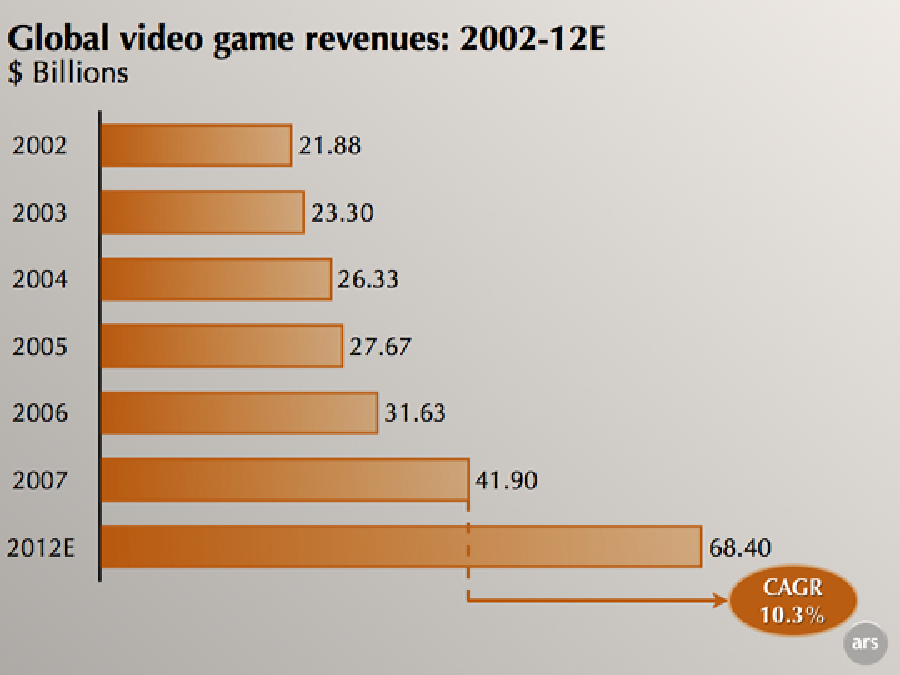
\includegraphics[width=14cm]{pic/bplan_02.pdf}
  \caption{Game sales}
  \label{fig:gamesale}
\end{figure}

Source: http://arstechnica.com/gaming/news/2008/06/gaming-expected-to-be-a-68-billion-business-by-2012.ars

\section{Touch screen devices}
Here are a few pictures of touch screen devices or tablets that are being presented in 2010. The tablet market is focused on consumer friendly tablets at the moment and we believe this is a great chance for us to get publicity for our electronic board games. We see it as offering yet another reason to buy a tablet in 2010.

\subsection{Apple iPad}

\begin{figure}[H]
  \centering
  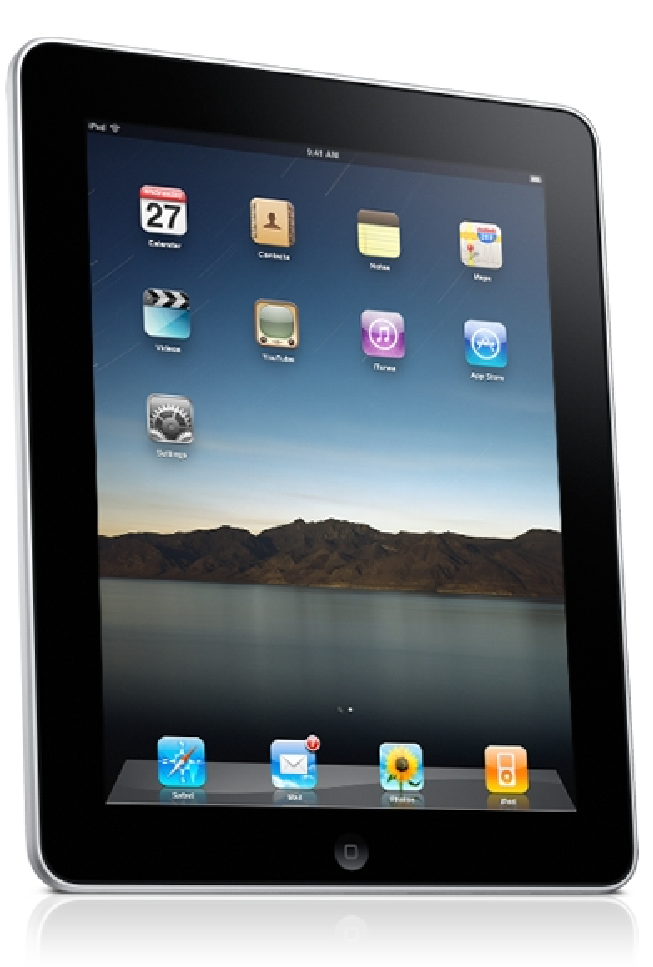
\includegraphics[width=4cm]{pic/bplan_03.pdf}
  \caption{Apple iPad}
  \label{fig:dev1}
\end{figure}

Source: \url{http://i.afterdawn.com/storage/pictures/apple_ipad_02.jpg}

\subsection{Microsoft tablet PC}

\begin{figure}[H]
  \centering
  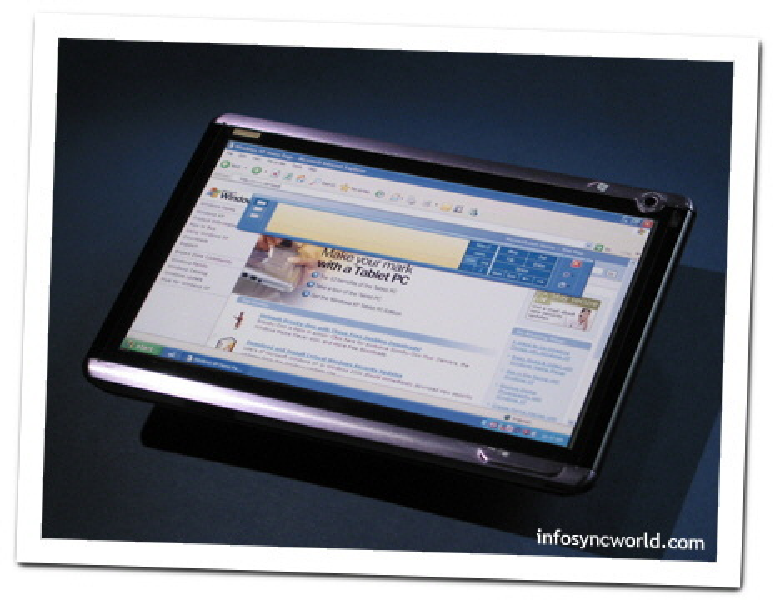
\includegraphics[width=7cm]{pic/bplan_04.pdf}
  \caption{Microsoft table PC}
  \label{fig:dev2}
\end{figure}

Source: \url{http://www.infosyncworld.net/2005/04/27/gfx/microsoft_tablet_pc_concept_01.jpg}

\subsection{HP Slate}

\begin{figure}[H]
  \centering
  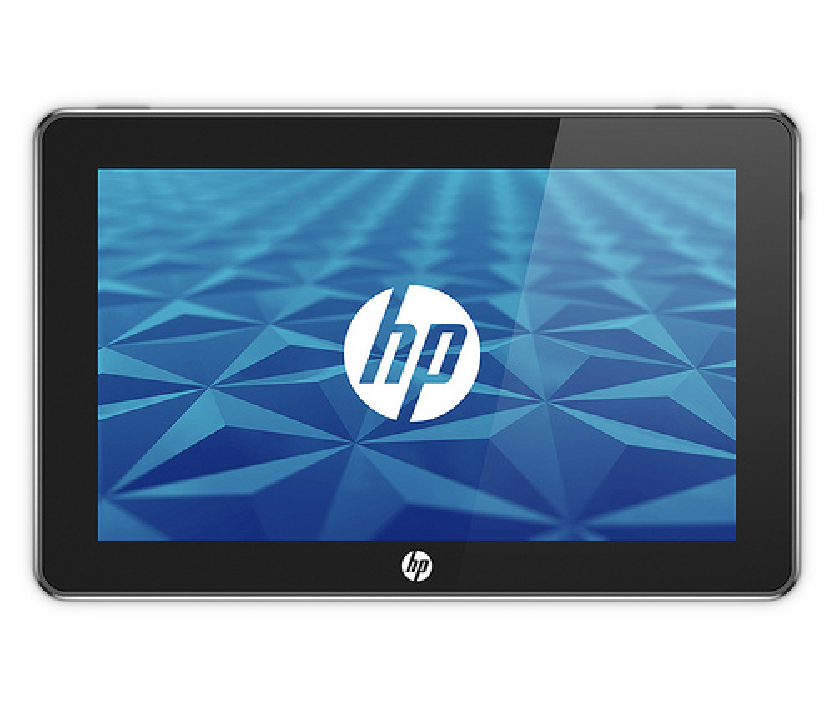
\includegraphics[width=7cm]{pic/bplan_05.pdf}
  \caption{HP Slate}
  \label{fig:dev3}
\end{figure}

Source: \url{http://mytechnews.info/b/wp-content/uploads/2010/01/hp-slate.jpg}

\subsection{Sony Dash}

\begin{figure}[H]
  \centering
  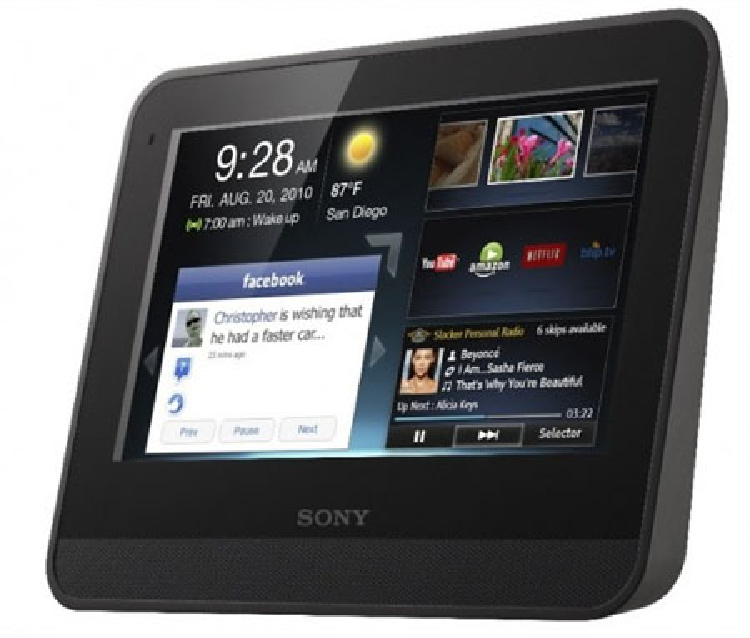
\includegraphics[width=7cm]{pic/bplan_06.pdf}
  \caption{HP Slate}
  \label{fig:dev4}
\end{figure}

Source: \url{http://www.pcfastlane.com/wp-content/uploads/2010/01/sony_dash1.jpg}

\pagebreak

\begin{thebibliography}{10}
\bibitem{CES} About.com: Portable Electronics. The CES 2010 Tablet roundup. 
Retrieved 17.2.2010 from \url{http://portables.about.com/od/otherdevices/tp/CES-2010-tablet-roundup.htm}
\bibitem{APP} Apple insider. First iPad estimates: 4 million units in year one, 8 million in 2011. 
Retrieved 6.2.2010 from \url{http://www.appleinsider.com/articles/10/01/27/first_ipad_estimates_4_million_units_in_year_one_8_million_in_2011.html}
\bibitem{ART} Ars Techinca. Gaming expected to be \$68 billion business by 2012. 
Retrieved 20.2.2010 from \url{http://arstechnica.com/gaming/news/2008/06/gaming-expected-to-be-a-68-billion-business-by-2012.ars}
\bibitem{DMW} Digital Media Wire, News. Report: Global Video Game sales to reach \$68,3 billion in 2012.
Retrieved 17.2.2010 from \url{http://www.dmwmedia.com/news/2008/06/18/report:-global-video-game-sales-reach-$68.3-billion-2012}
\bibitem{ESA}Entertainment Software Association. 2008. Sales, Demographic and usage data. Essential facts about the computer and video game industry. 
Retrieved 17.2.2010 from \url{http://www.theesa.com/facts/pdfs/ESA_EF_2008.pdf}
\bibitem{FS} Facebook Statistics. 
Retrieved 7.3.2010 from \url{http://www.facebook.com/press/info.php?statistics}
\bibitem{RiP} Recombu. Ipad board games: Apple has created a 'Jumanji platform'. 
Retrieved 4.2.2010 from \url{http://recombu.com/news/ipad-board-games-apple-has-created-a-jumanji-platform_M11370.html}
\bibitem{TINQ} The Inquirer. There are 75 million twitter users. 
Retrieved  7.3.2010 from \url{http://www.theinquirer.net/inquirer/news/1589058/there-75-million-twitter-users}
\bibitem{VEBG} Vizworld. Electronic board games. 
Retrieved 4.2.2010 from \url{http://www.vizworld.com/2010/01/electronic-board-games/}
\end{thebibliography}

\end{document}
